\begin{figure}[htb]
    \begin{center}
    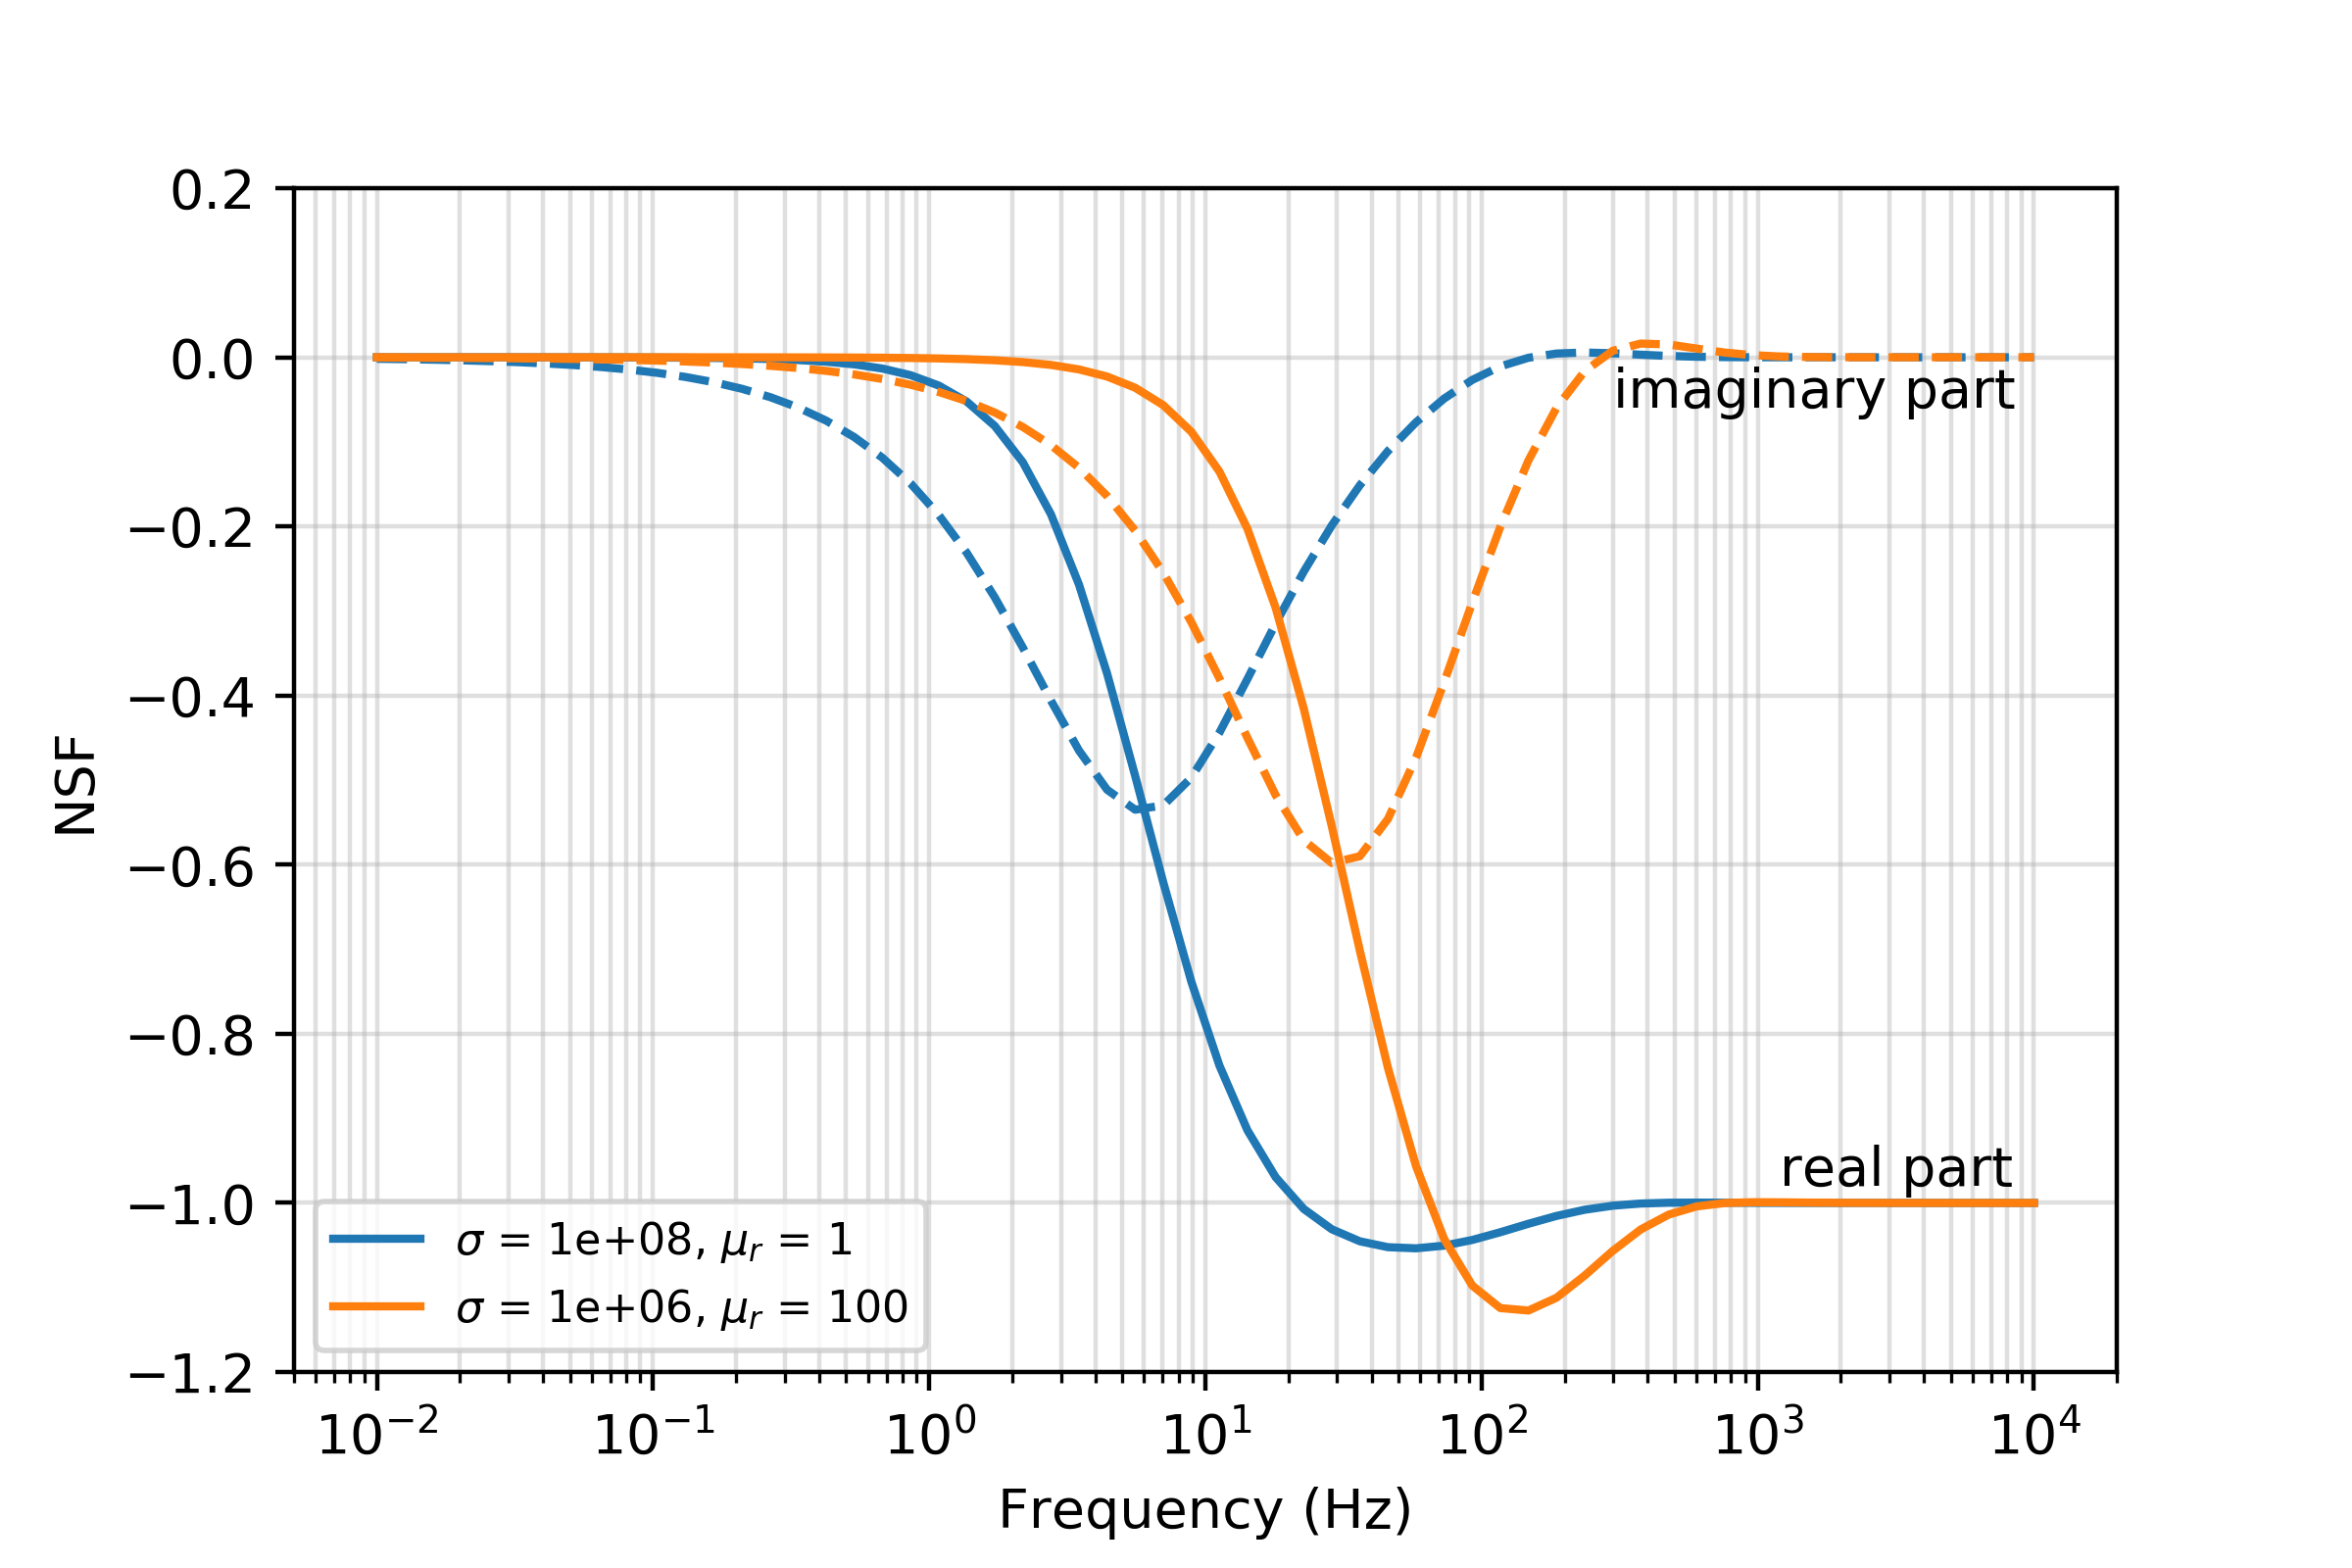
\includegraphics[width=0.6\columnwidth]{figures/fdemNSF.png}
    \end{center}
\caption{
    Normalized secondary field, NSF, as a function of frequency for two wells.
    The NSF is the ratio of the secondary vertical magnetic field with the primary magnetic field at the reciever location (z=-500m);
    the primary is defined as the whole-space primary.
}
\label{fig:fdemNSF}
\end{figure}
